\documentclass{polytech/polytech}
\schooldepartment{di}
\typereport{custom}
\typereportname{Ajout PRD}
\reportyear{2017-2018}
\title{Plateforme d'acquisition et de formatage temps réel multiflux TV Web}
\student[di5]{Romain}{ROUSSEAU}{romain.rousseau@etu.univ-tours.fr}
\academicsupervisor[di]{Mathieu}{DELALANDRE}{mathieu.delalandre@univ-tours.fr}


\resume{Ce projet consiste en l'élaboration d'une plateforme d'acquisition de flux TV Web en temps réel. L'objectif dans un premier temps consistera en l'affichage de plusieurs flux en simultané avant d'éventuellement faire évoluer l'application pour y faire figurer des éléments d'analyse d'images. Au travers de ce rapport, nous verrons la démarche, les objectifs liés à la mise en place d'une telle plateforme, l'architecture logicielle avec une structure en multi-threads, ainsi qu'un état de l'art sur ce domaine constante expansion et qui représente près de 80\% du trafic de données sur Internet.}

\motcle{Plateforme d'acquisition} 
\motcle{Flux de données} 
\motcle{Temps réel}
\motcle{Protocole de communication} 
\motcle{Télévision en ligne}


\abstract{This project consists in the making of acquisition platform of Live TV streams in real time. The first aim is to display multiple streams at the same time before evolving the platform to add elements of frame analysis. Through this document, we will see the approach, the goals link in the making of such a platform, the software architecture with a multi-threaded structure, as a state-of-the-art in this constantly evolving domain which represents almost 80\% of data traffic on the Internet.}

\keyword{Streaming Platform}
\keyword{Live Stream}
\keyword{Real Time}
\keyword{Communication Protocol}
\keyword{Online TV}


\addbibresource{bibliographie.bib}

%%%%%%%%%%%%%%%%%%%%%%%%%%%%%%%%%%%%%%%%%%%%%%%%%%%%%%%%%%%%%%%%%%%%%%%%%%%%%%%%%%%%%%%%%%%%%%%%%%%
%%%%%%%%%%%%%%%%%%%%%%%%%%%%%%%%%%%%%%%%%%%%%%%%%%%%%%%%%%%%%%%%%%%%%%%%%%%%%%%%%%%%%%%%%%%%%%%%%%%

\begin{document}


\chapter*{Introduction}


Alors qu’approche la fin du cursus à l’école Polytech Tours, se dresse le projet le plus important du parcours, le projet Recherche et Développement. Il s’étale sur l’ensemble de la cinquième année et représente une forme de synthèse des connaissances acquises lors des années d’études précédentes. Il permet de développer et d’approfondir son savoir sur un ou plusieurs champs de compétences spécifiques, afin de devenir un spécialiste du domaine choisi dans le cadre du projet. Ce projet est mené seul, sous la supervision du tuteur académique et avec l’aide d’un intervenant extérieur qui fait partie des initiateurs du sujet. Il permet ainsi de développer son autonomie en menant à bien un travail des prémices jusque, dans le meilleur des cas, à la production.

J’ai décidé de me consacrer à un sujet lié à un domaine en plein essor : le streaming. Ce sujet faisait partie de mes choix privilégiés lorsque j’ai vu la liste des sujets proposés. En effet, je regarde moi-même beaucoup de contenu audiovisuel par ce biais. J’ai pris pour habitude de regarder mes programmes télévisuelles préférés via mon ordinateur plutôt que par les usages traditionnelles avec une télévision depuis plusieurs années déjà, et il m’a paru intéressant de me pencher sur l’envers du décor et le fonctionnement de ces applications utilisées au quotidien par des milliers de personnes aujourd’hui.

Le but du projet est de réaliser une plateforme pour l’acquisition de flux de TV Web. Le contexte, les acteurs et les objectifs seront détaillés dans la première partie de ce rapport. En deuxième partie, nous retrouverons l’état de l’art et la veille technologique pour la plateforme, à savoir des informations sur les protocoles utilisés, les différentes librairies d’acquisition, les serveurs distribuant les flux, etc. La description générale du projet, avec son environnement, ses fonctionnalités et ses caractéristiques, sera dans la troisième partie de ce rapport. Le choix de présenter l’état de l’art et la veille technologique avant la description de la plateforme découle de la présentation des librairies et des protocoles utilisés, détaillés dans la deuxième partie. Il s’agit d’un choix qui permet d’accroître sa compréhension lorsque les descriptions fonctionnelles seront présentées. Enfin nous évoquerons les prémices d’analyse et de conception de la plateforme dans la dernière partie.

Des éléments complémentaires concernant notamment la gestion de projet via un diagramme
de Gantt sont disponibles en annexes.


\part{Contexte de la réalisation et cadre générale du projet}


\section{Contexte, enjeux et acteurs}

\section{Objectifs}

\section{Hypothèses}


\section{Base méthodologique}


\part{\'{E}tat de l'art et Veille technologique}


\chapter{\'{E}tat de l'art sur la télévision}

\section{Diffusion d'une chaîne de télévision}

\section{Réception de la télévision}

\subsection{Réception Hertzienne}

\subsection{Réception par satellite}

\subsection{Réception par câble}

\subsection{Service par contournement ou Over the Top (OTT)}


\chapter{La diffusion de flux en continu sur Internet}


\section{Principe générale du \textit{streaming}}


\section{Genèse du \textit{streaming} vidéo et évolution au fil du temps}

\section{Diffusion en flux adaptatif ou Adaptative Streaming}

\section{Les protocoles}

\subsection{HTTP}

\subsection{RTSP et RTSP 2.0}


\subsection{RTMP}

\subsection{MPEG-DASH, HLS, HDS et les nouveaux protocoles basés sur HTTP}

\section{Les formats de fichiers utilisés}


\chapter{Les chaînes de TV sur Internet en France}


\section{Critères de recherche}


\section{Résultats de l'étude}


\section{Tendances observées}


\section{Un mot sur le copyright}


\chapter{Les bibliothèques et logiciels d'acquisition}


\section{Les frameworks Windows (VfW, DirectShow, Media Foundation)}

\section{FFMPEG}


\section{libVLC et VLCJ}


\section{Streamlink}


\part{Description générale et analyse}


\chapter{Description générale}


\section{Environnement du projet}

\section{Caractéristiques des utilisateurs}


\section{Fonctionnalités du système}


\subsection{Séléction des chaînes via le fichier texte}

\subsection{Lancement en ligne de commande}

\subsection{Affichage des streams}

\section{Structure générale du système}


\subsection{La classe TVChannel}

\subsection{La classe MainLaunch}

\subsection{La classe MainControler}

\subsection{La classe StreamControler}

\subsection{La classe TextInputStreamControler}

\subsection{La classe StreamView}


\subsection{Lien entre les classes}


\chapter{Analyse des méthodes}



\part{Qualité de code et Tests de charges}


\chapter{Documentation et contrôle de qualité du code}


\section{Javadoc}


\section{Utilisation de SonarQube et SonarLint}

Pour le développement du site, nous nous sommes servis de l'outil de qualité de code \textit{SonarQube}. C'est un logiciel libre permettant de mesurer la qualité du code produit en se basant sur divers règles mises en place au préalable. Il peut détecter les bugs potentiels, les duplications de code, la couverture de code par les tests unitaires, et bien d'autres. Il supporte plus de 25 langages et s'adapte aux outils de build traditionnels (Ant, Maven, Gradle) ainsi qu'à certains IDE comme Eclipse. Il est aussi adaptable et personnalisable selon les besoins avec de nombreux plug-ins à disposition.

L'installation de SonarQube se fait très simplement. Il suffit de télécharger le programme, puis de lancer le script StartSonar.bat. Une instance de SonarQube sera lancée, et une fois que le message "\textit{SonarQube is up}" s'incrit sur la console comme on peut le voir sur la \autoref{fig:sonarcmd}, nous pouvons ouvrir la page du programme sur un navigateur. Par défaut, SonarQube utilise le port 9000 sur l'hôte local.


\begin{figure}
	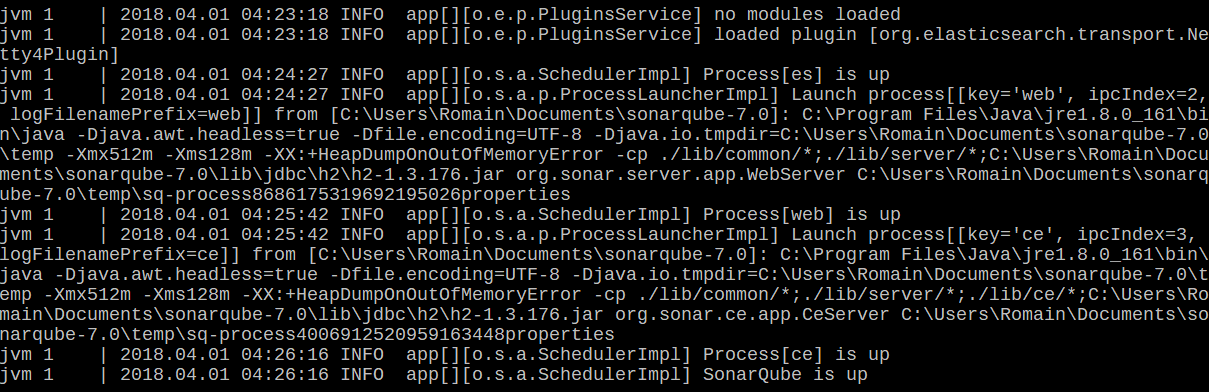
\includegraphics[scale=0.6]{sonarcmd.png}
	\caption{Lancement de l'instance SonarQube}
	\label{fig:sonarcmd}
\end{figure}


Maintenant que SonarQube est opérationnel, nous allons analyser notre projet. Dans un premier temps, nous regarderons l'application Angular. Dans notre cas, on souhaite que Sonar examine les fichiers \textit{typescript}. \'{E}tant donné que nous n'avons pas utilisé d'outils de build pour cette partie, nous avons installé un scanner sonar pour tout type de projet. Pour effectuer une analyse, il suffit de lancer depuis un terminal le script \textit{sonar-scanner} et de créer un fichier \textit{sonar-project.properties} comportant les détails concernant le projet, l'analyse s'effectuera par la suite. Le script va scanner tous les fichiers du dossier depuis lequel nous exécutons le programme et déterminera les éléments à modifier dans le code. Les résultats seront affichés dans l'instance SonarQube sur le navigateur internet.


Lors de notre première analyse sur l'application, nous avons eu les résultats suivants: 

\begin{figure}
	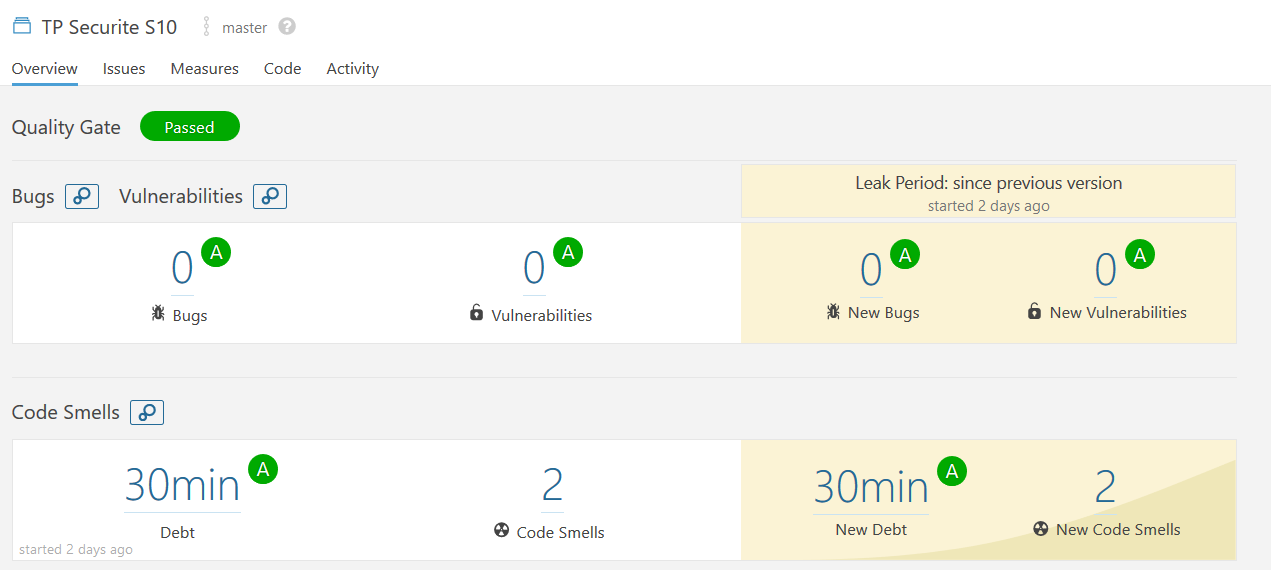
\includegraphics[scale=0.55]{sonarresult.png}
	\caption{Résultats de l'analyse Sonar}
	\label{fig:sonarresult}
\end{figure}

Nous pouvons remarquer que nous avons produit un code sans bug et sans vulnérabilités tout de suite, ce qui est déjà une très bonne chose. Il ne reste ainsi seulement qu'à corriger les deux erreurs détectées par Sonar pour avoir un code qui respecte les règles de Sonar. 


\chapter{Tests de charges}



\chapter*{Bilan et conclusion}


\appendix

\chapter{Interface Humain/Machine}

\chapter{Gestion de projet, diagramme de Gantt}


\chapter{Diagramme de classes}


\chapter{Diagramme de séquences}


\chapter{Guide d'installation et d'utilisation}


\section{Pré-requis}


La plateforme est destinée à fonctionner sur les machines de l’école. Il est nécessaire d'avoir une configuration réseau et matérielle solide si l'on souhaite faire fonctionner un maximum de chaînes en simultané sur l'application. La configuration minimale requise est la suivante :

\begin{itemize}
	\item Windows 7 Pro 64 bits
	\item Intel Xen CPU 3.06GHz
	\item 2 processeurs
	\item 4 Go de RAM
\end{itemize}


Pour la configuration réseau, la plateforme peut fonctionner sur un réseau Wi-Fi domicile mais la charge plafonne autour de 7 streams de qualité moyenne.


\section{Installations}

L'application nécessite plusieurs installations:

\subsection{Streamlink}

Streamlink est le logiciel en Python qui va prendre en charge les streams et qui va activer les flux à lire. Il existe plusieurs moyens de se procurer \textit{streamlink}, le plus simple est l'exécutable disponible à l'adresse : https://github.com/streamlink/streamlink/releases .

L'application fonctionne pour les versions 0.10.0 et supérieurs.

\subsection{VLC}

VLC est le logiciel permettant à l'application de visualiser les chaînes. Le programme  fonctionne avec la version 3.0.1 de VLC disponible à l'adresse suivante : https://get.videolan.org/vlc/3.0.1/win64/vlc-3.0.1-win64.exe


\subsection{Java Runtime Environment}

Le programme est un fichier jar qui fonctionne sur la version 8 de Java. Il est nécessaire pour le faire fonctionner de disposer du JRE 8 disponible à l'adresse : www.oracle.com/technetwork/java/javase/downloads/jre8-downloads-2133155.html


\section{Récupération du projet et fonctionnement}

Le projet se trouve sur le dépôt GitHub disponible à l'adresse suivante : https://github.com/RomainR37/streamPlatform

Une fois sur cette page, vous pouvez soit cloner le dépôt Git sur votre ordinateur, soit télécharger le dossier compressé en cliquant sur le bouton \textit{Clone or download} puis en sélectionnant son choix.

Après avoir récupérer le projet, vous pouvez l'exécuter en lancer une invit de commande Windows (en tapant Win+R au clavier puis \textit{cmd} dans le champ disponible). Une fois sur l'invit, dirigez vous vers le dossier du projet récupéré puis dans le dossier, allez dans le dossier \textit{target}. Il contient le fichier jar exécutable et un fichier texte exemple \textit{testStream.txt}. Pour lancer l'application avec le fichier \textit{testStream.txt} à disposition, la commande est la suivante : \javacode{java -jar streamPlatform-1.0.0-jar-with-dependencies.jar testStream.txt}. L'application se lancera.

\begin{figure}
	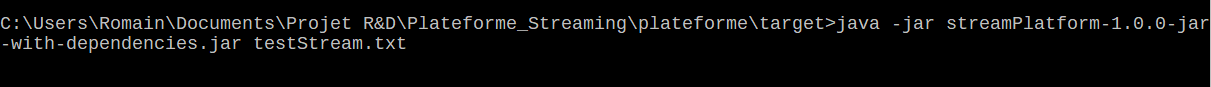
\includegraphics[scale=0.6]{images/cmdLancement.png}
	\caption{Commande de lancement du programme}
\end{figure}


\section{Fichier texte et syntaxe}

Il est possible de lancer l'application avec le fichier texte que l'on souhaite. Celui-ci pour fonctionner devra se situer dans le dossier \textit{target} également. Cependant le fichier doit respecter une convention de nommage. 


Une chaîne nécessite deux informations pour pouvoir fonctionner: son nom et l'adresse du site diffusant son stream. Dans le fichier texte que l'on veut lire, ces deux informations doivent transparaître séparées d'une tabulation. Vous pouvez voir l'exemple du fichier \textit{testStream.txt} ci-après:

\begin{figure}
	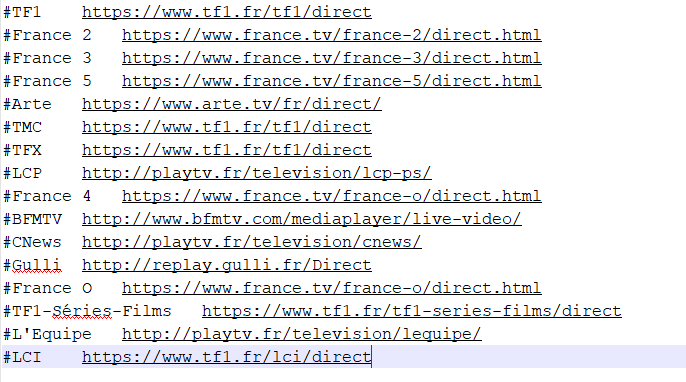
\includegraphics[scale=0.7]{images/testStream.png}
	\caption{Fichier texte exemple \textit{testStream}}
	\label{fig:fichier_texte}
\end{figure}

Ici sur la \autoref{fig:fichier_texte}, nous pouvons voir un \# avant une ligne. Il s'agit de la notation pour mettre une ligne en commentaire. Ainsi, le fichier \textit{testStream.txt} contient déjà une quinzaine de chaînes de télévision fonctionnelles, il suffit donc de supprimer les \# devant la chaîne que l'on veut visualiser. Néanmoins, il est possible de rajouter de nouvelles chaînes tant qu'elle respecte la convention. 

Certaines chaînes ne fonctionnent pas avec streamlink, et ne sont donc pas disponibles sur l'application. Par exemple, la version 0.11.0 de streamlink ne prend pas en charge les chaînes diffusées sur Dailymotion. Le problème sera sans doute réglé dans les prochaines versions ce qui rajoutera de nouvelles chaînes disponibles au visionnage. 


\section{Problèmes pouvant survenir}



\subsection{Pare-feu de Windows}

Un message du firewall peut apparaître au lancement de l'application. Cela est dû au script Python lancé par Streamlink. Il suffit que le firewall accepte les scripts pour que le fonctionnement se passe correctement. 


\subsection{Problèmes d'affichage}

Sur certaines machines, et en particulier sur les machines virtuelles de l'école, il est possible de constater des problèmes d'affichage des chaînes. On peut voir en effet sur des streams de bonne qualité, des problèmes au niveau des contours sur l'image (comme sur la \autoref{fig:pbAffichage}, en particulier à droite de l'image).


\begin{figure}
	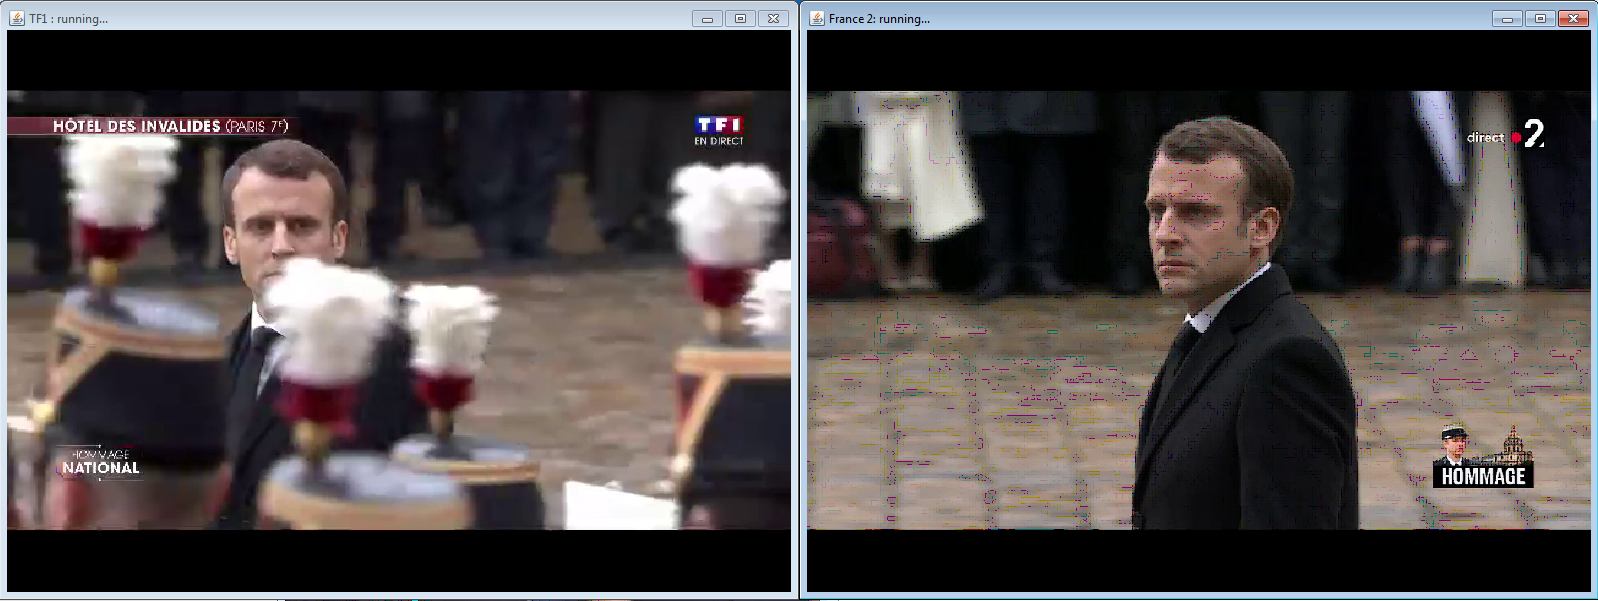
\includegraphics[scale=0.37]{images/imageQualite.png}
	\caption{Exemple de problèmes d'affichage}
	\label{fig:pbAffichage}
\end{figure}


Ces problèmes peuvent venir des configurations graphiques de la machine, notamment de DirectX. Néanmoins, lors des tests effectués sur machines Windows 10, il n'y avait aucun problème d'affichage, donc cela pourrait être des anciens systèmes Windows également.


\end{document}